% !TEX encoding = UTF-8 Unicode

\section{\large Introduction}

%%%%%%%%%%%%%%%%%%%%

\subsection{Background}

\begin{frame}[fragile,t]{Background}
	\begin{center}
	\begin{tabular}{m{0.4\textwidth} m{0.4\textwidth}}
	\center
\includegraphics[width=0.3\textwidth]{renaissance.jpg} & 
	\center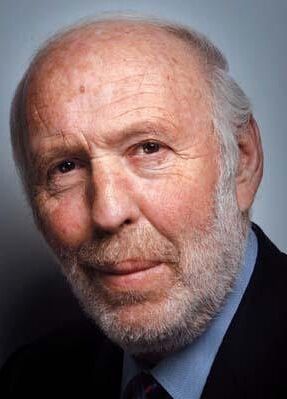
\includegraphics[width=1.5cm]{simmons.jpg}
	\end{tabular}
	\end{center}

	\begin{itemize}
	\item Quantitative finance analysis develops in China.
	\item Simple time series analysis techniques are incapable of capturing the market states.
	\item Dr.\,James H.~Simons implemented hidden Markov models (HMM)
		at Medallion Fund of Renaissance Technologies LLC.
	\end{itemize}

\end{frame}

%%%%%%%%%%%%%%%%%%%%

\subsection{Major Contributions and Key Spotlights}

\begin{frame}[fragile,t]{Major Contributions and Key Spotlights}
	% \begin{block}{Aim 1. System construction}
	% 	Construct the entire system for stock return series prediction, 
	% 	including data pre-processing, model construction and estimation, 
	% 	and eventually predictions with detailed analysis.
	% \end{block}

	% \begin{block}{Aim 2. Model estimation}
	% 	Estimate the HMM parameters in order to calibrate the model with accessible market data.
	% \end{block}

	% \begin{block}{Aim 3. Positive analysis}
	% 	Carry out empirical analysis on both Chinese and U.S. stock markets. 
	% 	Verify the effectiveness of the prediction system and provide detailed analysis and comparisons.
	% \end{block}

	% \begin{itemize}
	% 	\item \textbf{Aim 1. System construction} \\
	% 	Construct the entire system for stock return series prediction. \\
	% 	The system should include data pre-processing, model construction and estimation, 
	% 	and eventually predictions with detailed analysis.
	% 	\item \textbf{Aim 2. Model estimation} \\
	% 	Estimate the HMM parameters in order to calibrate the model with accessible market data.
	% 	\item \textbf{Aim 3. Positive analysis} \\
	% 	Carry out empirical analysis on both Chinese and U.S. stock markets. \\
	% 	Verify the effectiveness of the prediction system and provide detailed analysis and comparisons.
	% \end{itemize}
	\begin{block}{Major Contributions}
	\begin{itemize}
		\item 
		Construct the \alert{entire} system for stock return series prediction.
		\item 
		Carry out empirical analysis on both Chinese and U.S. stock markets,
		and among data with different observation frequencies.
	\end{itemize}
	\end{block}

	\begin{block}{Key Spotlights}
	\begin{itemize}
		\item 
		The system \alert{thoroughly encapsulates} the modules of data-preprocessing, 
		model initialization, parameters estimation and model calibration, 
		hidden states decoding and analysis, return series prediction and results output.
		\item 
		Hidden states analyses match common acknowledgements, 
		and the system performs well in \alert{adaptive} stock return series predictions.
	\end{itemize}
		
	\end{block}

\end{frame}

%%%%%%%%%%%%%%%%%%%%

\subsection{Thesis Organization}

\begin{frame}[fragile,t]{Thesis Organization}
	The thesis includes $7$ chapters and $2$ appendices:
	\begin{itemize}
	\item Chapter 1. Introduction
	\item Chapter 2. Preliminary Knowledge and Models
	\item Chapter 3. Hidden Markov Models
	\item Chapter 4. Stock Return Series Prediction System
	\item Chapter 5. Empirical Analysis on Stock Market Indices
	\item Chapter 6. Conclusion
	\item Chapter 7. Future Work
	\item Appendix A. Visualization of Simulated Prediction Results
	\item Appendix B. Model Realization Python Codes
	\end{itemize}

\end{frame}

%%%%%%%%%%%%%%%%%%%%

\section{\large Preliminary Knowledge}

%%%%%%%%%%%%%%%%%%%%

\subsection{Independent Mixture Distributions}

\begin{frame}[fragile]{Independent Mixture Distributions}
	Independent mixture distribution can deal with multi-modality of data. 
	Well-known mixture models include exponential distribuiton family models \cite{Hasselblad:1969bk},
	of which the most famous is Gaussian mixture model (GMM) \cite{Behboodian:1970hh}.
	
	An independent mixture distribution is formulated as:
		\[ p(x) = \sum_{i=1}^{m} \delta_ip_i(x), \quad\text{s.t.}\ \sum_{i=1}^{m} \delta_i = 1, \]
	where $p_i$ are component distributions and $\delta_i$ are component weights.
\end{frame}

%%%%%%%%%%%%%%%%%%%%

\subsection{Markov Chain}

\begin{frame}[fragile,t]{Markov Chain}
	\begin{itemize}
	\item Markovian property: 
		\[ \begin{aligned}
		& \prob{X_{t_n} \leq x_{n} \mid X_{t_1} = x_{1},X_{t_2} = x_{2},\dots,X_{t_{n-1}} = x_{n-1}} \\
		= & \prob{X_{t_n} \leq x_{n} \mid X_{t_{n-1}} = x_{n-1}}.
		\end{aligned} \]
	\item Homogeneity:
		\[ \prob{X_{m+k} = j \mid X_{m} = i} = \prob{X_{k} = j \mid X_{0} = i} := \gamma_{ij}^{(k)}. \]
	\item $k$-step transition probability matrix:
		\[ \bGamma^{(k)} = \left(\gamma_{ij}^{(k)} \right)_{i,j \in \hs}. \]
	\item Chapman-Kolmogorov equation:
		\[ \bGamma^{(t+u)} = \bGamma^{(t)}\bGamma^{(u)}. \]
	\end{itemize}
\end{frame}

%%%%%%%%%%%%%%%%%%%%

\subsection{K-Means Clustering}

\begin{frame}[fragile,t]{K-Means Clustering}
	Proposed by Stuart Lloyd in 1957 and by E.\,W.~Forgy in 1965 \cite{Forgy:1965cl} separately, 
	known as Lloyd-Forgy algorithm.
	The idea originates from vector quantization (VQ) in signal processing theories.

	\begin{itemize}
	\item Problem formulation:
		\[ \min_{\bS} \sum_{i=1}^{k}\sum_{\bx \in S_i} \norm{\bx - \bmu_i}^2, \]
	\item Algorithm:
		\begin{enumerate}
		\item assign step:
			\[ S_i^{(t)} = \left\{x_p \colon \norm{x_p-m_i^{(t)}}^2 \leq \norm{x_p-m_j^{(t)}}^2,
			\forall j,\ 1\leq j \leq k  \right\}. \]
		\item update step:
			\[ m_i^{(t+1)} = \frac{1}{\abs{S_i^{(t)}}} \sum_{x_j \in S_i^{(t)}} x_j. \]
		\end{enumerate}
	\end{itemize}
\end{frame}